\let\negmedspace\undefined
\let\negthickspace\undefined
\documentclass[journal,12pt,onecolumn]{IEEEtran}
\usepackage{gvv-book}
\usepackage{gvv}
\usepackage{mathtools}
\usepackage{amssymb,amsfonts,amsthm}
\usepackage{siunitx}
\usepackage{algorithmic}
\usepackage{graphicx}
\graphicspath{{./figs/}}
\usepackage{textcomp}
\usepackage{xcolor}
\usepackage{txfonts}
\usepackage{listings}
\usepackage{enumitem}
\usepackage{gensymb}
\usepackage{comment}
\usepackage{caption}
\usepackage{tkz-euclide}
\usepackage[latin1]{inputenc}
\usepackage{color}
\usepackage{array}
\usepackage{longtable}
\usepackage{calc}
\usepackage{multirow}
\usepackage{multicol}
\usepackage{hhline}
\usepackage{ifthen}
\usepackage{lscape}
\usepackage{tabularx}
\usepackage{float}
\usepackage[breaklinks=true]{hyperref}
\usepackage{cite}


\begin{document}

\title{
ASSIGNMENT 1: GATE PHYSICS }

\author{AI25BTECH11006 - Nikhila }
\maketitle

\vspace{6em} 

% ===== Constants Table =====


\noindent\textbf{\large Some useful physical constants, symbols and formulae}


\vspace{6em}

\begin{tabular}{ l l }
Speed of light in free space, $c$ & $3.0 \times 10^8\ \mathrm{m\,s^{-1}}$ \\
Atomic mass unit, $\mathrm{amu}$ & $1.66 \times 10^{-27}\ \mathrm{kg}$ \\
Avogadro's number, $N_A$ & $6.02 \times 10^{23}\ \mathrm{mole^{-1}}$ \\
Bohr magneton, $\mu_B$ & $9.27 \times 10^{-24}\ \mathrm{A\,m^2}$ \\
Boltzmann constant, $k_B$ & $1.38 \times 10^{-23}\ \mathrm{J\,K^{-1}}$ \\
Electron charge, $e$ & $1.60 \times 10^{-19}\ \mathrm{C}$ \\
Planck's constant, $h$ & $6.63 \times 10^{-34}\ \mathrm{J\,s}$ \\
Rest mass of electron, $m_e$ & $9.11 \times 10^{-31}\ \mathrm{kg}$ \\
Reduced Planck's constant, $\hbar$ & $1.05 \times 10^{-34}\ \mathrm{J\,s}$ \\
Permeability of free space, $\mu_0$ & $1.26 \times 10^{-6}\ \mathrm{N\,A^{-2}}$ \\
Permittivity of free space, $\varepsilon_0$ & $8.85 \times 10^{-12}\ \mathrm{C^2\,N^{-1}\,m^{-2}}$
\end{tabular}




\newpage

% ===== Questions =====
\begin{enumerate}[itemsep = 1em]

\item The eigenvalues of a matrix are $i$, $-2i$ and $3i$. The matrix is

\hfill{\brak{\text{GATE IN 20007}}}
\begin{enumerate}
\begin{multicols}{4}
\item unitary.
\item anti-unitary.
\item Hermitian.
\item anti-Hermitian.
\end{multicols}
\end{enumerate}

\item A space station moving in a circular orbit around the Earth goes into a new bound orbit by firing its engine radially outwards. This orbit is

\hfill{\brak{\text{GATE IN 20007}}}


\begin{enumerate}
\begin{multicols}{4}
\item a larger circle.
\item a smaller circle.
\item an ellipse.
\item a parabola.
\end{multicols}
\end{enumerate}

\item A power amplifier gives $150\ \mathrm{W}$ output for an input of $1.5\ \mathrm{W}$. The gain, in dB, is

\hfill{\brak{\text{GATE IN 20007}}}


\begin{enumerate}
\begin{multicols}{4}
\item 10
\item 20
\item 54
\item 100
\end{multicols}
\end{enumerate}

\item Four point charges are placed in a plane at the following positions:  
$+Q$ at $(1,0)$, $-Q$ at $(-1,0)$, $+Q$ at $(0,1)$, and $-Q$ at $(0,-1)$.  
At large distances the electrostatic potential due to this charge distribution will be dominated by the

\hfill{\brak{\text{GATE IN 20007}}}


\begin{enumerate}
\begin{multicols}{4}
\item monopole moment.
\item dipole moment.
\item quadrupole moment.
\item octopole moment.
\end{multicols}
\end{enumerate}

\item A charged capacitor $(C)$ is connected in series with an inductor $(L)$. When the displacement current reduces to zero, the energy of the LC circuit is

\hfill{\brak{\text{GATE IN 20007}}}


\begin{enumerate}
\begin{multicols}{2}
\item stored entirely in its magnetic field.
\item stored entirely in its electric field.
\item distributed equally among its electric and magnetic fields.
\item radiated out of the circuit.
\end{multicols}
\end{enumerate}


    
\item Match the following

\hfill{\brak{\text{GATE IN 20007}}}

\begin{tabular}{@{}ll}
P. Franck-Hertz experiment & 1. electronic excitation of molecules \\
Q. Hartree-Fock method     & 2. wave function of atoms \\
R. Stern-Gerlach experiment & 3. spin angular momentum of atoms \\
S. Franck-Condon principle & 4. energy levels in atoms
\end{tabular}

\vspace{0.5em}

\begin{multicols}{4}
(A) P-4, Q-2, R-3, S-1 \\
(B) P-1, Q-4, R-3, S-2 \\
(C) P-3, Q-2, R-4, S-1 \\
(D) P-4, Q-1, R-3, S-2
\end{multicols}


\item The wavefunction of a particle, moving in a one-dimensional time-independent potential $V(x)$, is given by
\[
\psi(x) = e^{-ax^2 + b}, \quad \text{where $a$ and $b$ are constants.}
\]
This means that the potential $V(x)$ is of the form

\hfill{\brak{\text{GATE IN 20007}}}


\begin{multicols}{2}
\begin{enumerate}
\item $V(x) \propto x$
\item $V(x) \propto x^2$
\item $V(x) = 0$
\item $V(x) \propto e^{-ax}$
\end{enumerate}
\end{multicols}


\item The $D_1$ and $D_2$ lines of Na ($3^2P_{1/2} \rightarrow 3^2S_{1/2}$, $3^2P_{3/2} \rightarrow 3^2S_{1/2}$) will split on the application of a weak magnetic field into

\hfill{\brak{\text{GATE IN 20007}}}


\begin{multicols}{2}
\begin{enumerate}
\item 4 and 6 lines respectively.
\item 3 lines each.
\item 6 and 4 lines respectively.
\item 6 lines each.
\end{enumerate}
\end{multicols}


\item In a He-Ne laser, the laser transition takes place in

\hfill{\brak{\text{GATE IN 20007}}}


\begin{multicols}{2}
\begin{enumerate}
\item He only.
\item Ne only.
\item Ne first, then in He.
\item He first, then in Ne.
\end{enumerate}
\end{multicols}


\item The partition function of a single gas molecule is $Z_a$. The partition function of $N$ such non-interacting gas molecules is then given by

\hfill{\brak{\text{GATE IN 20007}}}


\begin{multicols}{2}
\begin{enumerate}
\item $\dfrac{(Z_a)^N}{N!}$
\item $(Z_a)^N$
\item $N(Z_a)$
\item $\dfrac{(Z_a)^N}{N}$
\end{enumerate}
\end{multicols}


\item A solid superconductor is placed in an external magnetic field and then cooled below its critical temperature. The superconductor

\hfill{\brak{\text{GATE IN 20007}}}


\begin{multicols}{2}
\begin{enumerate}
\item retains its magnetic flux because the surface current supports it.
\item expels out its magnetic flux because it behaves like a paramagnetic material.
\item expels out its magnetic flux because it behaves like an anti-ferromagnetic material.
\item expels out its magnetic flux because the surface current induces a field in the direction opposite to the applied magnetic field.

\end{enumerate}
\end{multicols}


\item A particle with energy $E$ is in a time-independent double well potential as shown in the figure.

\begin{figure}[h!]
    \centering
    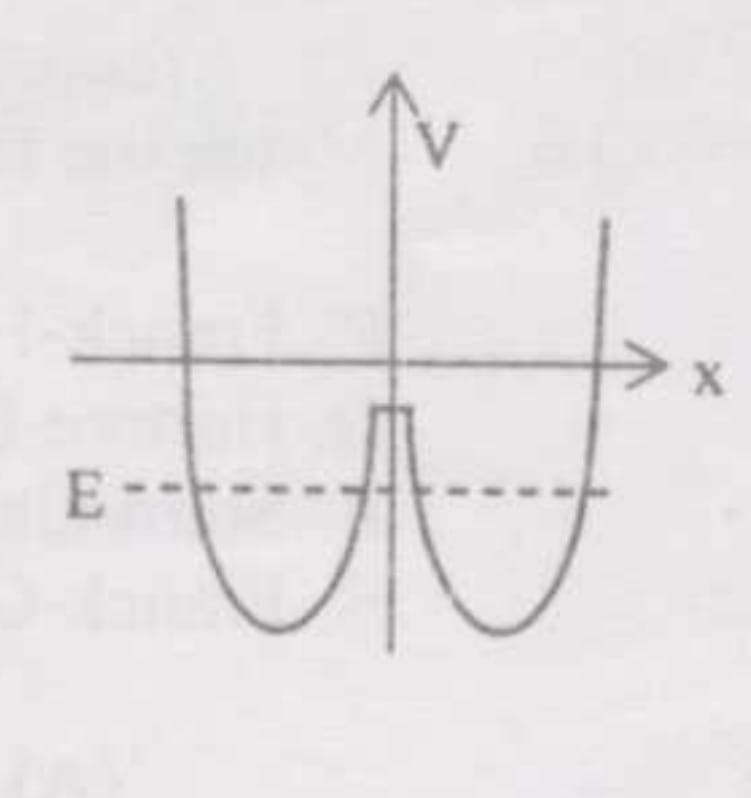
\includegraphics[width=0.25\textwidth]{fig1.jpeg}
    \caption{}
    \label{fig:fig1.jpeg}
\end{figure}

Which of the following statements about the particle is \textbf{NOT} correct?

\hfill{\brak{\text{GATE IN 20007}}}

\begin{enumerate}
    \item The particle will always be in a bound state.
    \item The probability of finding the particle in one well will be time-dependent.
    \item The particle will be confined to any one of the wells.
    \item The particle can tunnel from one well to the other, and back.
\end{enumerate}



\item It is necessary to apply quantum statistics to a system of particles if

\hfill{\brak{\text{GATE IN 20007}}}

\begin{enumerate}
    \item There is substantial overlap between the wavefunctions of the particles.
    \item The mean free path of the particles is comparable to the inter-particle separation.
    \item The particles have identical mass and charge.
    \item The particles are interacting.
\end{enumerate}


\item When liquid oxygen is poured down close to a strong bar magnet, the oxygen stream is

\hfill{\brak{\text{GATE IN 20007}}}

\begin{enumerate}
    \item Repelled towards the lower field because it is diamagnetic.
    \item Attracted towards the higher field because it is diamagnetic.
    \item Repelled towards the lower field because it is paramagnetic.
    \item Attracted towards the higher field because it is paramagnetic.
\end{enumerate}


\item Fission fragments are generally radioactive as

\hfill{\brak{\text{GATE IN 20007}}}

\begin{enumerate}
    \item They have excess of neutrons.
    \item They have excess of protons.
    \item They are products of radioactive nuclides.
    \item Their total kinetic energy is of the order of $200\,\mathrm{MeV}$.
\end{enumerate}


\item In a typical $npn$ transistor the doping concentrations in emitter, base and collector regions are $C_E, C_B$ and $C_C$ respectively. These satisfy the relation,

\hfill{\brak{\text{GATE IN 20007}}}

\begin{enumerate}
    \item $C_E > C_C > C_B$
    \item $C_E > C_B > C_C$
    \item $C_C > C_B > C_E$
    \item $C_E = C_C > C_B$
\end{enumerate}


\item The allowed states for He ($2p^2$) configuration are

\hfill{\brak{\text{GATE IN 20007}}}

\begin{enumerate}
    \item $^1S_0,\, ^3S_1,\, ^1P_1,\, ^3P_{0,1,2},\, ^1D_2,\, ^3D_{1,2,3}$
    \item $^1S_0,\, ^3P_{0,1,2},\, ^1D_2$
    \item $^1P_1,\, ^3P_{0,1,2}$
    \item $^1S_0,\, ^1P_1$
\end{enumerate}


\item The energy levels of a particle of mass $m$ in a potential of the form
\[
V(x) = 
\begin{cases}
\infty, & x \leq 0 \\
\frac{1}{2}m\omega^2 x^2, & x > 0
\end{cases}
\]
are given, in terms of quantum number $n = 0,1,2,\dots$, by

\hfill{\brak{\text{GATE IN 20007}}}

\begin{enumerate}
    \item $\left(n + \frac{1}{2}\right)\hbar\omega$
    \item $\left(2n + \frac{1}{2}\right)\hbar\omega$
    \item $\left(2n + \frac{3}{2}\right)\hbar\omega$
    \item $\left(n + \frac{3}{2}\right)\hbar\omega$
\end{enumerate}


\item The electromagnetic field due to a point charge must be described by lienard-wechert potentials when

\hfill{\brak{\text{GATE IN 20007}}}

\begin{enumerate}
    \item The point charge is highly accelerated.
    \item the electric and magnetic fields are not perpendicular.
    \item the point charge is moving with velocity close to that of light.
    \item the calculation is done for the radiation zone.
\end{enumerate}


\item The strangeness quantum number is conserved in

\hfill{\brak{\text{GATE IN 20007}}}

\begin{enumerate}
    \item strong, weak and electromagnetic interactions
    \item weak and electromagnetic interactions only.
    \item strong and weak interaction only.
    \item strong and electromagnetic interactions only.
\end{enumerate}


\item the eigenvalues and eigenvectors of the matrix \myvec{5 & 4\\1 & 2} are 

\hfill{\brak{\text{GATE IN 20007}}}

\begin{multicols}{2}
\begin{enumerate}
    \item 6, 1 and \myvec{4\\1},\myvec{1\\-1}
    \item 2, 5 and \myvec{4\\1},\myvec{1\\-1}
    \item 6, 1 and \myvec{1\\4},\myvec{1\\-1}
    \item 2, 5 and \myvec{1\\4},\myvec{1\\-1}
    \end{enumerate}
\end{multicols}


\item A vector field is defined everywhere as 
\begin{align*}
 \vec{F} = \frac{y^2}{L}\hat{i} + z\hat{k}   
\end{align*}.  The net flux of $\vec{F}$ associated with a cube of side L, with one vertex at the origin and sides along the positive X, Y, Z axes is

\hfill{\brak{\text{GATE IN 20007}}}

\begin{multicols}{4}
\begin{enumerate}
    \item $2L^{3}$
    \item $4L^{3}$
    \item $8L^{3}$
    \item $10L^{3}$
    \end{enumerate}
\end{multicols}


\item If $\vec{r} = x\hat{i} + y\hat{j}$ , then

\hfill{\brak{\text{GATE IN 20007}}}

\item Consider a vector $\vec{p} = 2\hat{i} + 3\hat{j} + 2\hat{k}$ in the coordinate system $(\hat{i},\hat{j},\hat{k})$. The axes are rotated anti-clockwise about the $Y$ axis by an angle of $60\degree$. The vector $\vec{p}$ in the rotated coordinate system $(\hat{i}',\hat{j}',\hat{k}')$ is

\hfill{\brak{\text{GATE IN 2007}}}

\begin{enumerate}

\item $(1-\sqrt{3})\hat{i}' + 3\hat{j}' + (1+\sqrt{3})\hat{k}'$
\item $(1+\sqrt{3})\hat{i}' + 3\hat{j}' + (1-\sqrt{3})\hat{k}'$
\item $(1-\sqrt{3})\hat{i}' + (3+\sqrt{3})\hat{j}' + 2\hat{k}'$
\item $(1-\sqrt{3})\hat{i}' + (3-\sqrt{3})\hat{j}' + 2\hat{k}'$

\end{enumerate}

\vspace{2em}


\item The contour integral $\oint \frac{dz}{z^2+a^2}$ is to be evaluated on a circle of radius $2a$ centered at the origin. It will have contributions only from the points

\hfill{\brak{\text{GATE IN 2007}}}


\begin{enumerate}

\item $\frac{1+i}{\sqrt{2}}a$ and $\frac{1-i}{\sqrt{2}}a$
\item $ia$ and $-ia$
\item $ia, -ia, \frac{-1+i}{\sqrt{2}}a$ and $\frac{-1-i}{\sqrt{2}}a$
\item $\frac{1+i}{\sqrt{2}}a, \frac{-1+i}{\sqrt{2}}a, \frac{-1-i}{\sqrt{2}}a$ and $\frac{1-i}{\sqrt{2}}a$

\end{enumerate}

\vspace{2em}

\item Inverse Laplace transform of $\frac{s+1}{s^2-4}$ is

\hfill{\brak{\text{GATE IN 2007}}}

\begin{enumerate}
\begin{multicols}{4}
\item $\cos 2x + \frac{1}{2} \sin 2x$
\item $\cos x + \frac{1}{2} \sin x$
\item $\cosh x + \frac12 \sinh x$
\item $\cosh 2x + \frac12 \sinh 2x$
\end{multicols}
\end{enumerate}

\item The points, where the series solution of the Legendre differential equation  
$(1-x^2)\frac{d^2y}{dx^2} - 2x\frac{dy}{dx} + \frac{3}{2}\left(\frac{3}{2}+1\right)y=0$  
will diverge, are located at

\hfill{\brak{\text{GATE IN 2007}}}

\begin{enumerate}
\begin{multicols}{4}
\item $0$ and $1$
\item $0$ and $-1$
\item $-1$ and $1$
\item $\frac{3}{2}$ and $\frac{5}{2}$
\end{multicols}
\end{enumerate}

\vspace{3em}

\item Solution of the differential equation $x\frac{dy}{dx} + y = x^4$, with the boundary condition that $y=1$ at $x=1$, is

\hfill{\brak{\text{GATE IN 2007}}}

\begin{enumerate}
\begin{multicols}{4}
\item $y = 5x^4 - 4$
\item $y = x^4 + \frac{4x}{5}$
\item $y = \frac{4x^4}{5} + \frac{1}{5x}$
\item $y = x^4 + \frac{4}{5x}$
\end{multicols}
\end{enumerate}

\item Match the following:

\begin{table}[H]
\centering
\caption{Matching list for Question \theenumi}
\label{tab:q29}
\begin{tabular}{|l|l|}
\hline
P. rest mass & 1. timelike vector \\
Q. charge & 2. Lorentz invariant \\
R. four-momentum & 3. tensor of rank 2 \\
S. electromagnetic field & 4. conserved and Lorentz invariant \\
\hline
\end{tabular}
\end{table}

\hfill{\brak{\text{GATE IN 2007}}}

\vspace{1em}

\begin{enumerate}
\begin{multicols}{2}
\item P-2, Q-4, R-3, S-1
\item P-4, Q-2, R-1, S-3
\item P-2, Q-4, R-1, S-3
\item P-4, Q-2, R-3, S-1
\end{multicols}
\end{enumerate}

\vspace{2em}

\item The moment of inertia of a uniform sphere of radius $r$ about an axis passing through its centre is given by $\frac{2}{5}\left(\frac{4\pi r^3}{3}\rho\right)$.

A rigid sphere of uniform mass density $\rho$ and radius $R$ has two smaller spheres of radius $R/2$ hollowed out of it, as shown in the figure. The moment of inertia of the resulting body about the $Y$-axis is

\begin{figure}[ht!]
    \centering
    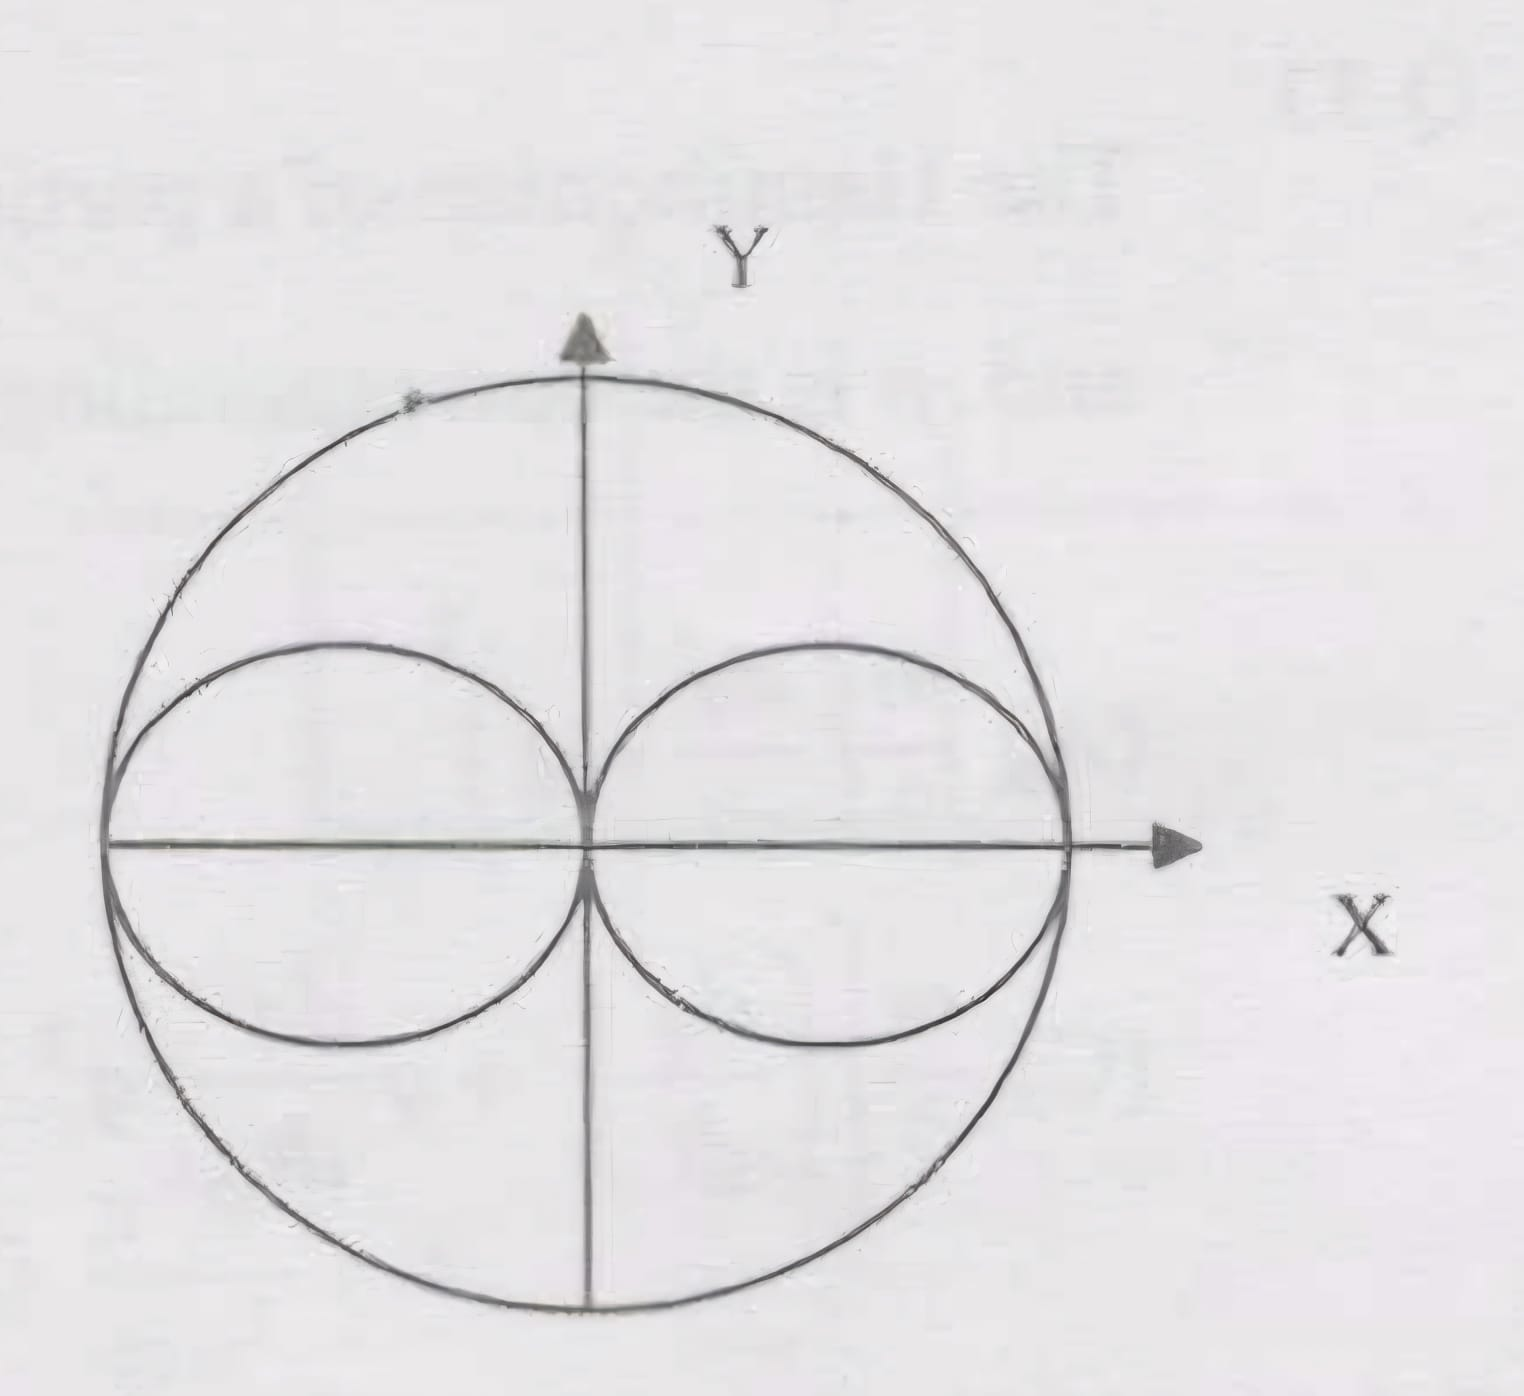
\includegraphics[width=0.25\textwidth]{fig2.jpeg}
    \caption{}
    \label{fig:fig2.jpeg}
\end{figure}

Which of the following statements about the particle is \textbf{NOT} correct?

\hfill{\brak{\text{GATE IN 2007}}}


\hfill{\brak{\text{GATE IN 20007}}}

\vspace{2em}

\begin{enumerate}
\begin{multicols}{4}
    \item $\frac{\pi \rho R^{5}}{4}$
    \item $\frac{5 \pi \rho R^{5}}{12}$
    \item $\frac{7 \pi \rho R^{5}}{12}$.
    \item $\frac{3 \pi \rho R^{5}}{4}$
\end{multicols}
\end{enumerate}

\item The Lagrangian of a particle of mass $m$ is 
\[
L = \frac{m}{2} \left[ \left( \frac{dx}{dt} \right)^2 + \left( \frac{dy}{dt} \right)^2 + \left( \frac{dz}{dt} \right)^2 \right]
- \frac{\nu}{2} \left( x^2 + y^2 \right) + W' \sin(\omega t),
\]
where $\nu, W'$ and $\omega$ are constants. The conserved quantities are:

\hfill{\brak{\text{GATE IN 20007}}}

\begin{enumerate}
\item energy and $z$-component of linear momentum only.
\item energy and $z$-component of angular momentum only.
\item 2-components of both linear and angular momenta only.
\item energy and $z$-components of both linear and angular momenta.
\end{enumerate}

\item  Three particles of mass $m$ each situated at $x_{1}(t)$, $x_{2}(t)$ and $x_{3}(t)$ respectively are connected by two springs of spring constant $k$ and un-stretched length $l$. The system is free to oscillate only in one dimension along the straight line joining all the three particles. The Lagrangian of the system is:

\hfill{\brak{\text{GATE IN 20007}}}

\begin{enumerate}
\item $L = \frac{m}{2} \left[ \left( \frac{dx_{1}}{dt} \right)^{2} + \left( \frac{dx_{2}}{dt} \right)^{2} + \left( \frac{dx_{1}}{dt} \right)^{2} \right] 
- \frac{k}{2} \left( x_{1} - x_{2} - l \right)^{2} + \frac{k}{2} \left( x_{1} - x_{2} - l \right)^{2}$

\item $L = \frac{m}{2} \left[ \left( \frac{dx_{1}}{dt} \right)^{2} + \left( \frac{dx_{2}}{dt} \right)^{2} + \left( \frac{dx_{1}}{dt} \right)^{2} \right] 
- \frac{k}{2} \left( x_{1} - x_{9} - l \right)^{2} + \frac{k}{2} \left( x_{1} - x_{2} - l \right)^{2}$

\item $L = \frac{m}{2} \left[ \left( \frac{dx_{1}}{dt} \right)^{2} + \left( \frac{dx_{2}}{dt} \right)^{2} + \left( \frac{dx_{1}}{dt} \right)^{2} \right] 
- \frac{k}{2} \left( x_{1} - x_{2} + l \right)^{2} - \frac{k}{2} \left( x_{1} - x_{2} + l \right)^{2}$

\item $L = \frac{m}{2} \left[ \left( \frac{dx_{1}}{dt} \right)^{2} + \left( \frac{dx_{2}}{dt} \right)^{2} + \left( \frac{dx_{3}}{dt} \right)^{2} \right] 
- \frac{k}{2} \left( x_{1} - x_{2} - l \right)^{2} - \frac{k}{2} \left( x_{1} - x_{2} - l \right)^{2}$
\end{enumerate}

\item The Hamiltonian of a particle is $H = \frac{p^{2}}{2m} + pq$ where $q$ is the generalized coordinate and $p$ is the corresponding canonical momentum. The Lagrangian is:

\hfill{\brak{\text{GATE IN 20007}}}

\begin{enumerate}
\item $\frac{m}{2} \left( \dot{q} + q \right)^{2}$
\item $\frac{m}{2} \left( \dot{q} - q \right)^{2}$
\item $\frac{m}{2} \left[ \dot{q}^{2} + q \dot{q} - q^{2} \right]$
\item $\frac{m}{2} \left[ \dot{q}^{2} - q \dot{q} + q^{2} \right]$
\end{enumerate}

\item A toroidal coil has $N$ closely-wound turns. Assume the current through the coil to be $I$ and the toroid is filled with a magnetic material of relative permeability $\mu_{r}$. The magnitude of magnetic induction $\vec{B}$ inside the toroid, at a radial distance $r$ from the axis, is given by:

\hfill{\brak{\text{GATE IN 20007}}}

\begin{enumerate}
\begin{multicols}{2}
\item $\mu_{r} \mu_{0} \frac{N I}{r}$
\item $\mu \, \mu_{0} \frac{N I}{r}$
\item $\frac{\mu_{r} \mu_{0} N I}{2 \pi r}$
\item $2\pi \, \mu_{r} \mu_{0} \frac{N I}{r}$
\end{multicols}
\end{enumerate}

\item Can the following scalar and vector potentials describe an electromagnetic field?
\begin{align}
\phi(x,y,z) &= 3xyz - 4r \\
\vec{A}(\vec{x},t)  &= (2x - \omega t) \, \hat{i} + (y - 2z) \, \hat{j} + (z-2xe^{i\omega t}) \, \hat{k}  
\end{align}

\hfill{\brak{\text{GATE IN 20007}}}

\begin{enumerate}
\item Yes, in the Coulomb gauge.
\item Yes, in the Lorentz gauge.
\item Yes, provided $\omega = 0$.
\item No.
\end{enumerate}


\item An electromagnetic wave $\tilde{E}(z,t) = E_{0} \cos(\alpha \nu t - kz) \, \hat{z}$ is traveling in free space and crosses a disc of radius $2\,\text{m}$ placed perpendicular to the $z$-axis. If $E_{z} = 60 \ \mathrm{V \, m^{-1}}$, the average power, in Watt, crossing the disc along the $z$-direction is:

\hfill{\brak{\text{GATE IN 20007}}}

\begin{enumerate}
\begin{multicols}{4}
\item 30
\item 60
\item 120
\item 270
\end{multicols}
\end{enumerate}

\item For a particle of mass $m$ in a one-dimensional harmonic oscillator potential of the form  $V(x) = \frac{1}{2} m \omega^{2} x^{2}$. the first excited energy eigenstate is  $\psi(x) = x \, e^{ -\alpha \omega x^{2} }$ The value of $\alpha$ is:

\hfill{\brak{\text{GATE IN 20007}}}

\begin{enumerate}
\begin{multicols}{4}
\item $\frac{m \omega}{4 \hbar}$
\item $\frac{m \omega}{3 \hbar}$
\item $\frac{m \omega}{2 \hbar}$
\item $\frac{2 m \omega}{3 \hbar}$
\end{multicols}
\end{enumerate}


\item If $[x, p] = i \hbar$, the value of $[x^{3}, p]$ is:

\hfill{\brak{\text{GATE IN 20007}}}

\begin{enumerate}
\begin{multicols}{4}
\item $2 i \hbar x^{2}$
\item $-\frac{2}{\hbar} x^{2}$
\item $3 i \hbar x^{2}$
\item $-3 i \hbar x^{2}$
\end{multicols}
\end{enumerate}

\item There are only three bound states for a particle of mass m  in a one-dimensional potential well of the form shown in the figure. The depth $V_0$ of the potential satisfies

\begin{figure}[ht!]
    \centering
    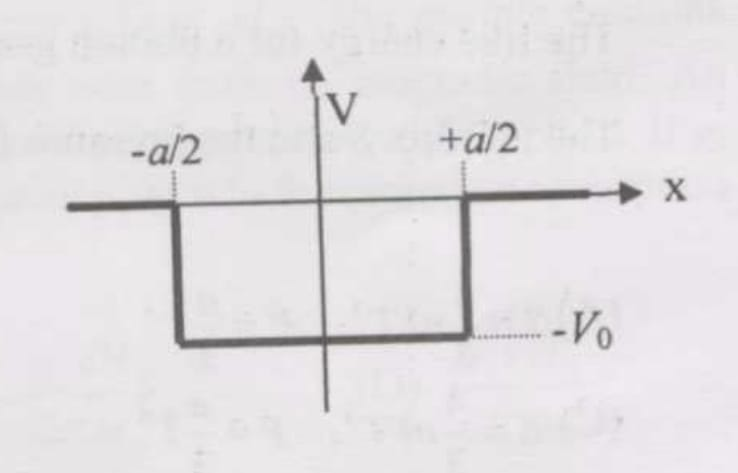
\includegraphics[width=0.25\textwidth]{fig3.jpeg}
    \caption{}
    \label{fig:fig3.jpeg}
\end{figure}

\hfill{\brak{\text{GATE IN 20007}}}

\begin{enumerate}
\begin{multicols}{2}
\item $\frac{m}{2} \left( \frac{dq}{dt} + q \right)^{2}$
\item $\frac{m}{2} \left( \frac{dq}{dt} - q \right)^{2}$
\item $\frac{m}{2} \left[ \left( \frac{dq}{dt} \right)^{2} + q \frac{dq}{dt} - q^{2} \right]$
\item $\frac{m}{2} \left[ \left( \frac{dq}{dt} \right)^{2} - q \frac{dq}{dt} + q^{2} \right]$
\end{multicols}{}
\end{enumerate}

\item A toroidal coil has $N$ closely-wound turns. Assume the current through the coil to be $I$ and the toroid is filled with a magnetic material of relative permeability $\mu_{r}$. The magnitude of magnetic induction $\vec{B}$ inside the toroid, at a radial distance $r$ from the axis, is given by:

\hfill{\brak{\text{GATE IN 20007}}}

\begin{enumerate}
\begin{multicols}{2}
\item $\mu_{r} \mu_{0} \frac{N I}{r}$
\item $\mu \, \mu_{0} \frac{N I}{r}$
\item $\frac{\mu_{r} \mu_{0} N I}{2 \pi r}$
\item $2\pi \, \mu_{r} \mu_{0} \frac{N I}{r}$
 \end{multicols}
\end{enumerate}

\item An electromagnetic wave $\tilde{E}(z,t) = E_{0} \cos(\alpha \nu t - kz) \, \hat{z}$ is traveling in free space and crosses a disc of radius $2\,\text{m}$ placed perpendicular to the $z$-axis. If $E_{z} = 60 \ \mathrm{V \, m^{-1}}$, the average power, in Watt, crossing the disc along the $z$-direction is:

\hfill{\brak{\text{GATE IN 20007}}}

\begin{enumerate}
\begin{multicols}{4}
\item 30
\item 60
\item 120
\item 270
\end{multicols}
\end{enumerate}

\item For a particle of mass $m$ in a one-dimensional harmonic oscillator potential of the form  $V(x) = \frac{1}{2} m \omega^{2} x^{2}$ , the first excited energy eigenstate is $\psi(x) = x \, e^{ -\alpha \omega x^{2} }$. The value of $\alpha$ is:

\hfill{\brak{\text{GATE IN 20007}}}

\begin{enumerate}
\begin{multicols}{4}
\item $\frac{m \omega}{4 \hbar}$
\item $\frac{m \omega}{3 \hbar}$
\item $\frac{m \omega}{2 \hbar}$
\item $\frac{2 m \omega}{3 \hbar}$
\end{multicols}
\end{enumerate}

\item If $[x, p] = i \hbar$, the value of $[x^{3}, p]$ is:

\hfill{\brak{\text{GATE IN 20007}}}

\begin{enumerate}
\begin{multicols}{4}
\item $2 i \hbar x^{2}$
\item $-\frac{2}{\hbar} x^{2}$
\item $3 i \hbar x^{2}$
\item $-3 i \hbar x^{2}$
\end{multicols}
\end{enumerate}

\item The free energy for a photon gas is given by $F = -\frac{\alpha}{3} \nu T^{4}$, where $\alpha$ is a constant. The entropy $S$ and the pressure $P$ of the photon gas are

\hfill{\brak{\text{GATE IN 2007}}}
\begin{enumerate}
\begin{multicols}{2}
\item $S = \frac{4}{3}aV T, \quad P = \frac{a}{3}T^{4}$
\item $S = \frac{1}{3}aV T^{4}, \quad P = \frac{4a}{3}T^{3}$
\item $S = \frac{4}{3}aV T^{3}, \quad P = \frac{a}{3}T^{3}$
\item $S = \frac{1}{3}aV T^{3}, \quad P = \frac{4a}{3}T^{4}$
\end{multicols}
\end{enumerate}

\item A system has energy levels $E_{0}, \ 2E_{0}, \ 3E_{0}, \dots$ where the excited states are triply degenerate. Four non-interacting bosons are placed in this system. If the total energy of these bosons is $5E_{0}$, the number of microstates is

\hfill{\brak{\text{GATE IN 2007}}}
\begin{enumerate}
\begin{multicols}{4}
\item $2$
\item $3$
\item $4$
\item $5$
\end{multicols}
\end{enumerate}

\item In accordance with the selection rules for electric dipole transitions, the $4^{3}P_{1}$ state of helium can decay by photon emission to the states

\hfill{\brak{\text{GATE IN 2007}}}
\begin{enumerate}
\begin{multicols}{2}
\item $2^{1}S_{0}, \ 2^{1}P_{1}, \ 3^{1}D_{2}$
\item $3^{1}P_{1}, \ 3^{1}D_{2}, \ 3^{1}S_{0}$
\item $3^{3}P_{2}, \ 3^{3}D_{3}, \ 3^{3}P_{0}$
\item $2^{3}S_{1}, \ 3^{3}D_{2}, \ 3^{3}D_{1}$
\end{multicols}
\end{enumerate}

\item If an atom is in the $^{3}D_{3}$ state, the angle between its orbital and spin angular momentum vectors \brak{\vec{L} and \vec{S}}is

\hfill{\brak{\text{GATE IN 2007}}}
\begin{enumerate}
\begin{multicols}{4}
\item $\cos\left(\frac{1}{\sqrt{3}}\right)$
\item $\cos^{-1}\left(\frac{2}{\sqrt{3}}\right)$
\item $\cos^{-1}\left(\frac{1}{2}\right)$
\item $\cos\left(\frac{\sqrt{3}}{2}\right)$
\end{multicols}
\end{enumerate}

\item The hyperfine structure of Na $(3^{2}P_{3/2})$ with nuclear spin $I = \frac{3}{2}$ has

\hfill{\brak{\text{GATE IN 2007}}}
\begin{enumerate}
\begin{multicols}{4}
\item $1$ state
\item $2$ states
\item $3$ states
\item $4$ states
\end{multicols}
\end{enumerate}

\item The allowed rotational energy levels of a rigid hetero-nuclear diatomic molecule are expressed as $\varepsilon_{J} = BJ(J+1)$ where $B$ is the rotational constant and $J$ is a rotational quantum number.

In a system of such diatomic molecules of reduced mass $\mu$, some of the atoms of one element are replaced by a heavier isotope, such that the reduced mass changes to $1.05\mu$. In the rotational spectrum of the system, the shift in the spectral line corresponding to a transition $J=4 \to J=5$ is

\hfill{\brak{\text{GATE IN 2007}}}
\begin{enumerate}
\begin{multicols}{4}
\item $0.475B$
\item $0.50B$
\item $0.95B$
\item $1.0B$
\end{multicols}
\end{enumerate}

\item The number of fundamental vibrational modes of CO$_{2}$ molecule is

\hfill{\brak{\text{GATE IN 2007}}}
\begin{enumerate}

\item Four: $2$ Raman active and $2$ infrared active
\item Four: $1$ Raman active and $3$ infrared active
\item Three: $1$ Raman active and $2$ infrared active
\item Three: $2$ Raman active and $1$ infrared active

\end{enumerate}


\item A piece of paraffin is placed in a uniform magnetic field $H_{0}$. The sample contains hydrogen nuclei of mass $m_{p}$ which interact only with the external magnetic field. An additional oscillating magnetic field is applied to observe resonance absorption. If $g$ is the g-factor of the hydrogen nucleus, the frequency at which resonance absorption takes place is given by

\hfill{\brak{\text{GATE IN 2007}}}
\begin{enumerate}
\begin{multicols}{4}
\item $\frac{3 g_{1} e H_{0}}{2 \pi m_{p}}$
\item $\frac{3 g_{j} e H_{0}}{4 \pi m_{p}}$
\item $\frac{g_{z} e H_{0}}{2 \pi m_{p}}$
\item $\frac{S_{r} e H_{q}}{4 \pi m_{p}}$
\end{multicols}
\end{enumerate}

\item The solid phase of an element follows van der Waals bonding with inter-atomic potential $V(r) = - \frac{P}{r^5} + \frac{Q}{r^{12}}$, where $P$ and $Q$ are constants. The bond length can be expressed as

\hfill{\brak{\text{GATE IN 2007}}}
\begin{enumerate}
\begin{multicols}{4}
\item $\left(\frac{2P}{Q}\right)^{-6}$
\item $\left(\frac{P}{Q}\right)^{-6}$
\item $\left(\frac{P}{2Q}\right)^{-6}$
\item $\left(\frac{P}{Q}\right)^{-6}$
\end{multicols}
\end{enumerate}

\item Consider the atomic packing factor (APF) of the following crystal structures:

P. Simple Cubic

Q. Body Centred Cubic

R. Face Centred Cubic

S. Diamond

T. Hexagonal Close Packed

Which two of the above structures have equal APF?

\hfill{\brak{\text{GATE IN 2007}}}
\begin{enumerate}
\begin{multicols}{4}
\item P and Q
\item S and T
\item R and S
\item R and T
\end{multicols}
\end{enumerate}

\item In a powder diffraction pattern recorded from a face-centred cubic sample using x-rays, the first peak appears at $30^\circ$. The second peak will appear at

\hfill{\brak{\text{GATE IN 2007}}}
\begin{multicols}{4}
\begin{enumerate}

\item $32.8^\circ$
\item $33.7^\circ$
\item $34.8^\circ$
\item $35.3^\circ$

\end{enumerate}
\end{multicols}


\vspace{8em}

\item Variation of electrical resistivity $\rho$ with temperature T of three solids is sketched \brak{on different scales} in the figure, as curves P, Q and R.\\

Which one of the following statements describes the variations most appropriately?

\hfill{\brak{\text{GATE IN 2007}}}

\begin{figure}[ht!]
    \centering
    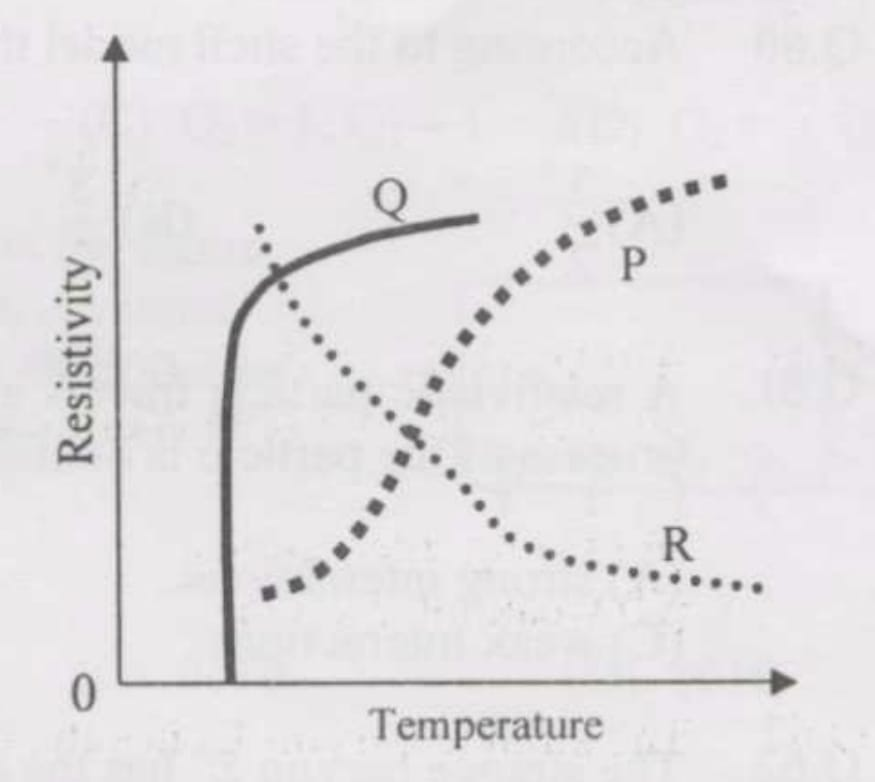
\includegraphics[width=0.25\textwidth]{fig4.jpeg}
    \caption{}
    \label{fig:fig4.jpeg}
\end{figure}

\begin{enumerate}
    \item P is a superconductor, and R for a semiconductor.
    \item Q is a superconductor, and P for a conductor.
    \item Q is a superconductor, and R for a conductor.
    \item R is a superconductor, and P for a conductor.
    
\end{enumerate}

\item An extrinsic semiconductor sample of cross-section $A$ and length $L$ is doped in such a way that the doping concentration varies as $N_D(x) = N_0 \exp(-x/L)$. Assume that the mobility of the majority carriers remains constant. The resistance $R$ of the sample is given by:  

\hfill{\brak{\text{GATE IN 2007}}}

\begin{multicols}{2}
\begin{enumerate}
    \item $R = \dfrac{L}{A \mu N_0} \left[\exp(1)-1\right]$
    \item $R = \dfrac{L}{\mu \pi r N_0} \left[\exp(1)-1\right]$
    \item $R = \dfrac{L}{A \epsilon N_0} \left[\exp(-1)-1\right]$
    \item $R = \dfrac{L}{A \mu N_g}$
\end{enumerate}
\end{multicols}

\item A ferromagnetic mixture of iron and copper having $75\%$ atoms of Fe exhibits a saturation magnetization of $1.3 \times 10^6 \ \mathrm{A/m}$. Assume that the total number of atoms per unit volume is $8 \times 10^{28} \ \mathrm{m}^{-3}$. The magnetic moment of an iron atom, in terms of the Bohr magneton, is:  

\hfill{\brak{\text{GATE IN 2007}}}

\begin{multicols}{2}
\begin{enumerate}
    \item 1.7
    \item 2.3
    \item 2.9
    \item 3.8
\end{enumerate}
\end{multicols}

\item Half-life of a radio-isotope is $4 \times 10^4$ years. If there are $10^3$ radioactive nuclei in a sample today, the number of such nuclei in the sample $4 \times 10^5$ years ago were:  

\hfill{\brak{\text{GATE IN 2007}}}

\begin{multicols}{2}
\begin{enumerate}
    \item $1.28 \times 10^5$
    \item $2.56 \times 10^5$
    \item $5.12 \times 10^5$
    \item $1.024 \times 10^6$
\end{enumerate}
\end{multicols}

\item In the deuterium + tritium (D + T) fusion, more energy is released compared to deuterium + deuterium (D + D) fusion because:  

\hfill{\brak{\text{GATE IN 2007}}}

\begin{multicols}{2}
\begin{enumerate}
    \item Tritium is radioactive
    \item More nucleons participate in fusion
    \item The Coulomb barrier is lower for the D+T system than D+D system
    \item The reaction product He is more tightly bound
\end{enumerate}
\end{multicols}

\item According to the shell model, the ground state spin of the $^{17}$O nucleus is:  

\hfill{\brak{\text{GATE IN 2007}}}

\begin{multicols}{2}
\begin{enumerate}
    \item $3/2^+$
    \item $5/2^+$
    \item $3/2^-$
    \item $5/2^-$
\end{enumerate}
\end{multicols}

\item A relativistic particle travels a length of $3 \times 10^{-3}$ m in air before decaying. The decay process of the particle is dominated by:  

\hfill{\brak{\text{GATE IN 2007}}}

\begin{multicols}{2}
\begin{enumerate}
    \item Strong interactions
    \item Electromagnetic interactions
    \item Weak interactions
    \item Gravitational interactions
\end{enumerate}
\end{multicols}

\item The strange baryon $\Xi^-$ has the quark structure:  

\hfill{\brak{\text{GATE IN 2007}}}

\begin{multicols}{4}
\begin{enumerate}
    \item $uds$
    \item $uud$
    \item $uus$
    \item $u\bar{s}$
\end{enumerate} 
\end{multicols}


\item A neutron scatters elastically from a heavy nucleus. The initial and final states off the neutron have the

\hfill{\brak{\text{GATE IN 2007}}}

\begin{enumerate}
    \item same energy.
    \item same energy and linear momentum.
    \item same energy and angular momentum.
    \item same linear and angular momentum.
\end{enumerate}


\vspace{13em}

\item The circuit shown is based on ideal operational amplifiers. It acts as a 

\hfill{\brak{\text{GATE IN 2007}}}

\begin{figure}[ht!]
    \centering
    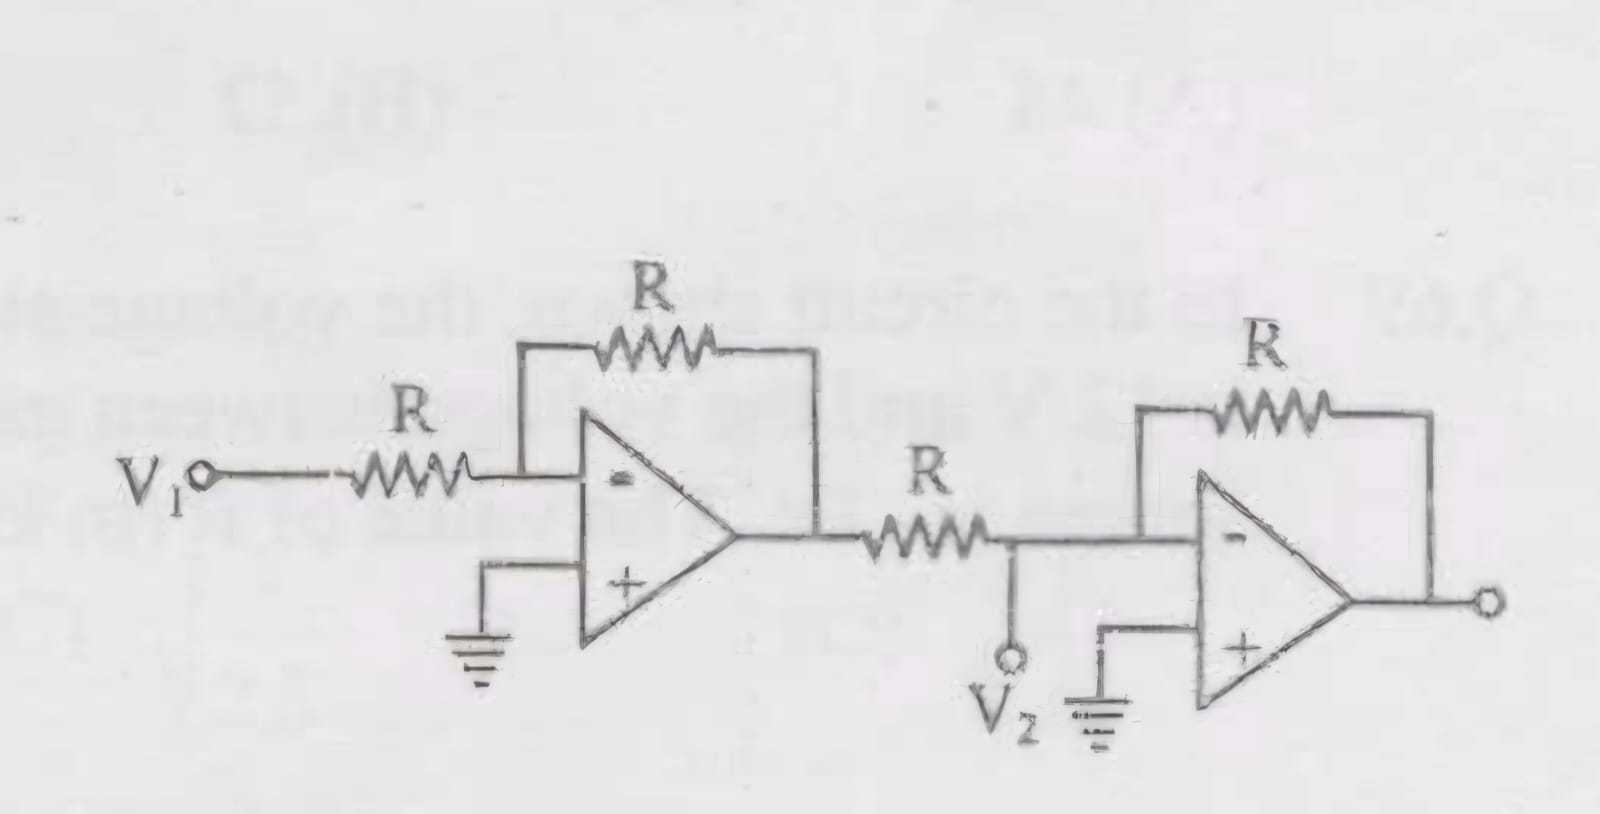
\includegraphics[width=0.5\textwidth]{fig5.jpeg}
    \caption{}
    \label{fig:fig5.jpeg}
\end{figure}

\begin{multicols}{4}
\begin{enumerate}
    \item subtractor
    \item buffer amplifier
    \item adder
    \item divider
\end{enumerate} 
\end{multicols}

\item Identify the function F generated by the logic network shown

\hfill{\brak{\text{GATE IN 2007}}}

\begin{figure}[ht!]
    \centering
    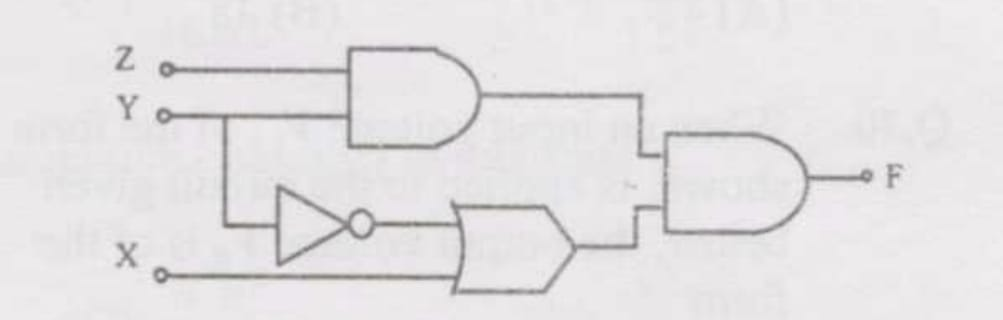
\includegraphics[width=0.5\textwidth]{fig6.jpeg}
    \caption{}
    \label{fig:fig6.jpeg}
\end{figure}

\begin{multicols}{4}
\begin{enumerate}
    \item F = \brak{X + Y}Z
    \item F = Z + Y +YX
    \item ZY\brak{Y + X}
    \item XYZ
\end{enumerate} 
\end{multicols}

\item In the circuit shown, the ports $Q_1$ and $Q_2$ are in the state $Q_1$ = 1, $Q_2$ = 0. The circuit is now subjected to two complete clock pulses. The state of these ports now becomes

\hfill{\brak{\text{GATE IN 2007}}}

\begin{figure}[ht!]
    \centering
    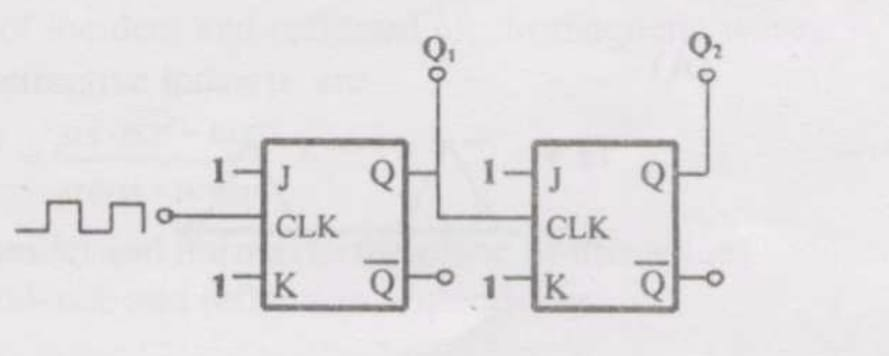
\includegraphics[width=0.5\textwidth]{fig7.jpeg}
    \caption{}
    \label{fig:fig7.jpeg}
\end{figure}

\begin{multicols}{4}
\begin{enumerate}
    \item $Q_2$ = 1, $Q_1$ = 0
    \item $Q_2$ = 0, $Q_1$ = 1
    \item $Q_2$ = 1, $Q_1$ = 1
    \item $Q_2$ = 0, $Q_1$ = 0
\end{enumerate} 
\end{multicols}

\vspace{4em}

\item The registers $Q_D$, $Q_C$, $Q_B$ and $Q_A$ shown in the figure are initially in the state 1010 respectively. An input sequence SI = 0101 is applied. After two clock pulses, the state of the shift registers is

\hfill{\brak{\text{GATE IN 2007}}}

\begin{figure}[ht!]
    \centering
    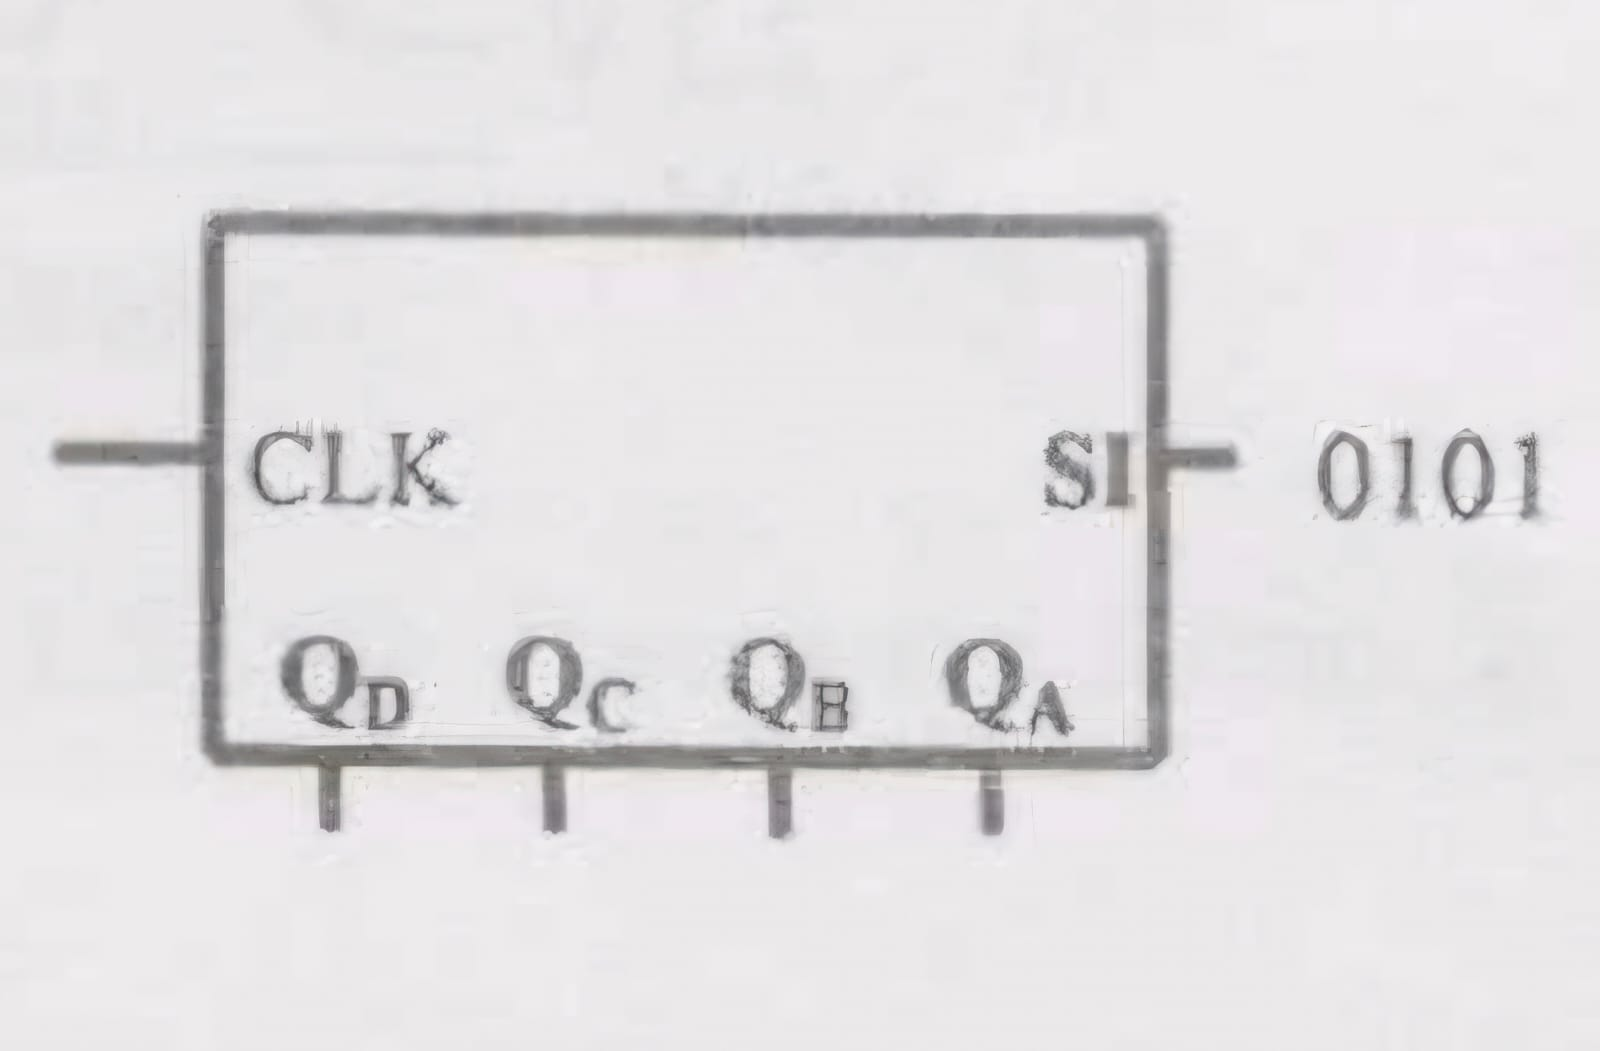
\includegraphics[width=0.4\textwidth]{fig8.jpeg}
    \caption{}
    \label{fig:fig8.jpeg}
\end{figure}

\begin{multicols}{4}
\begin{enumerate}
    \item 1001
    \item 0100
    \item 0110
    \item 1010
\end{enumerate} 
\end{multicols}


\item For the circuit shown, the potential difference in volts across $R_L$ is

\hfill{\brak{\text{GATE IN 2007}}}

\begin{figure}[ht!]
    \centering
    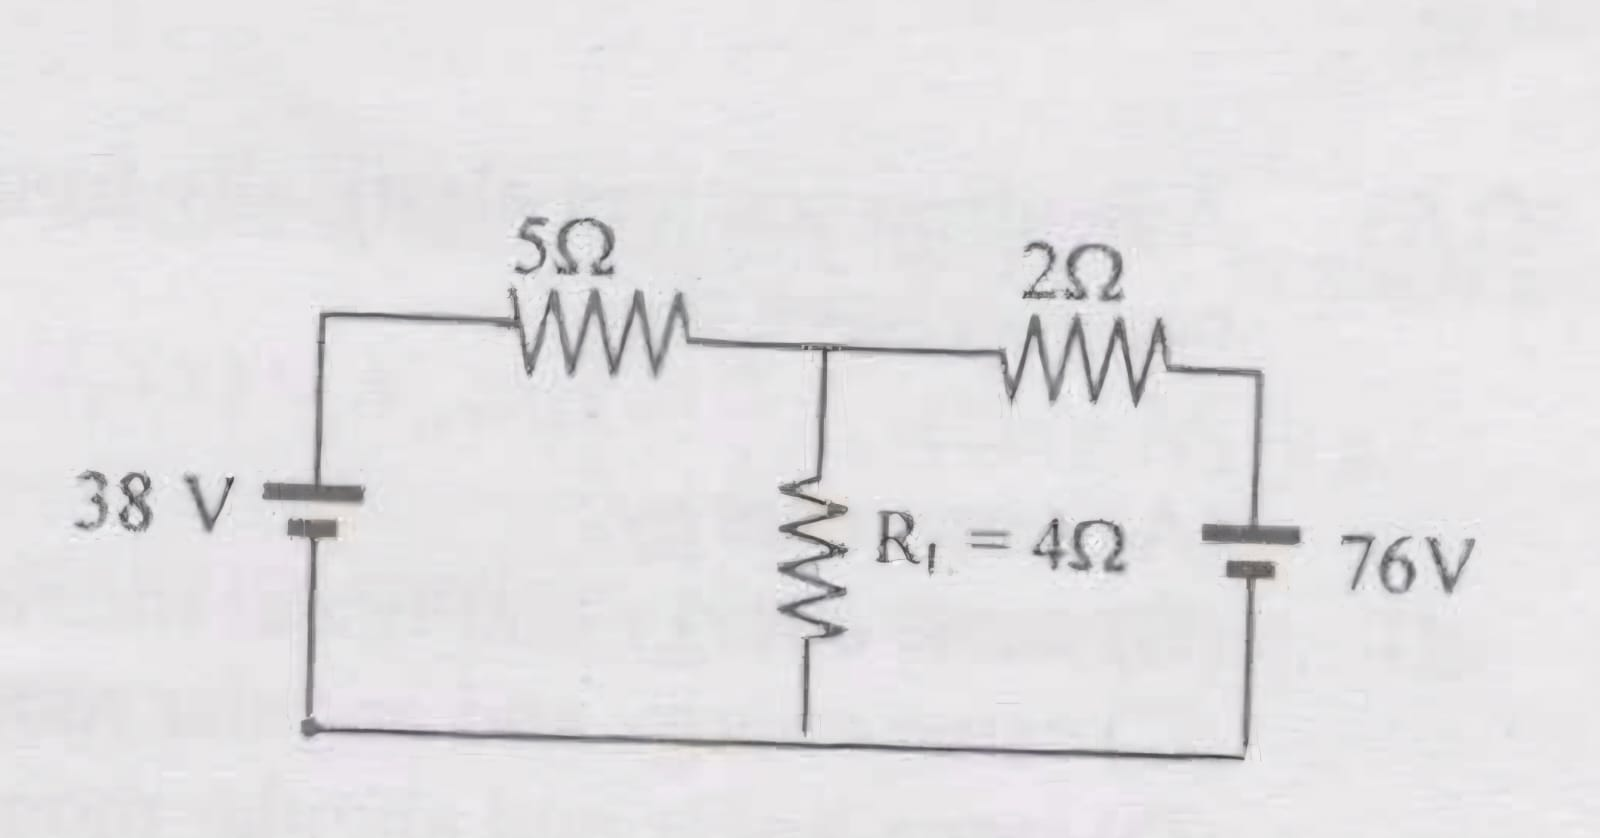
\includegraphics[width=0.4\textwidth]{fig9.jpeg}
    \caption{}
    \label{fig:fig9.jpeg}
\end{figure}

\begin{multicols}{4}
\begin{enumerate}
    \item 48
    \item 52
    \item 56
    \item 65
\end{enumerate} 
\end{multicols}


\item In the circuit shown, the voltage at test point P is 12 V and the voltage between gate and source is -2V. The value of R in k\ohm is

\hfill{\brak{\text{GATE IN 2007}}}

\begin{figure}[ht!]
    \centering
    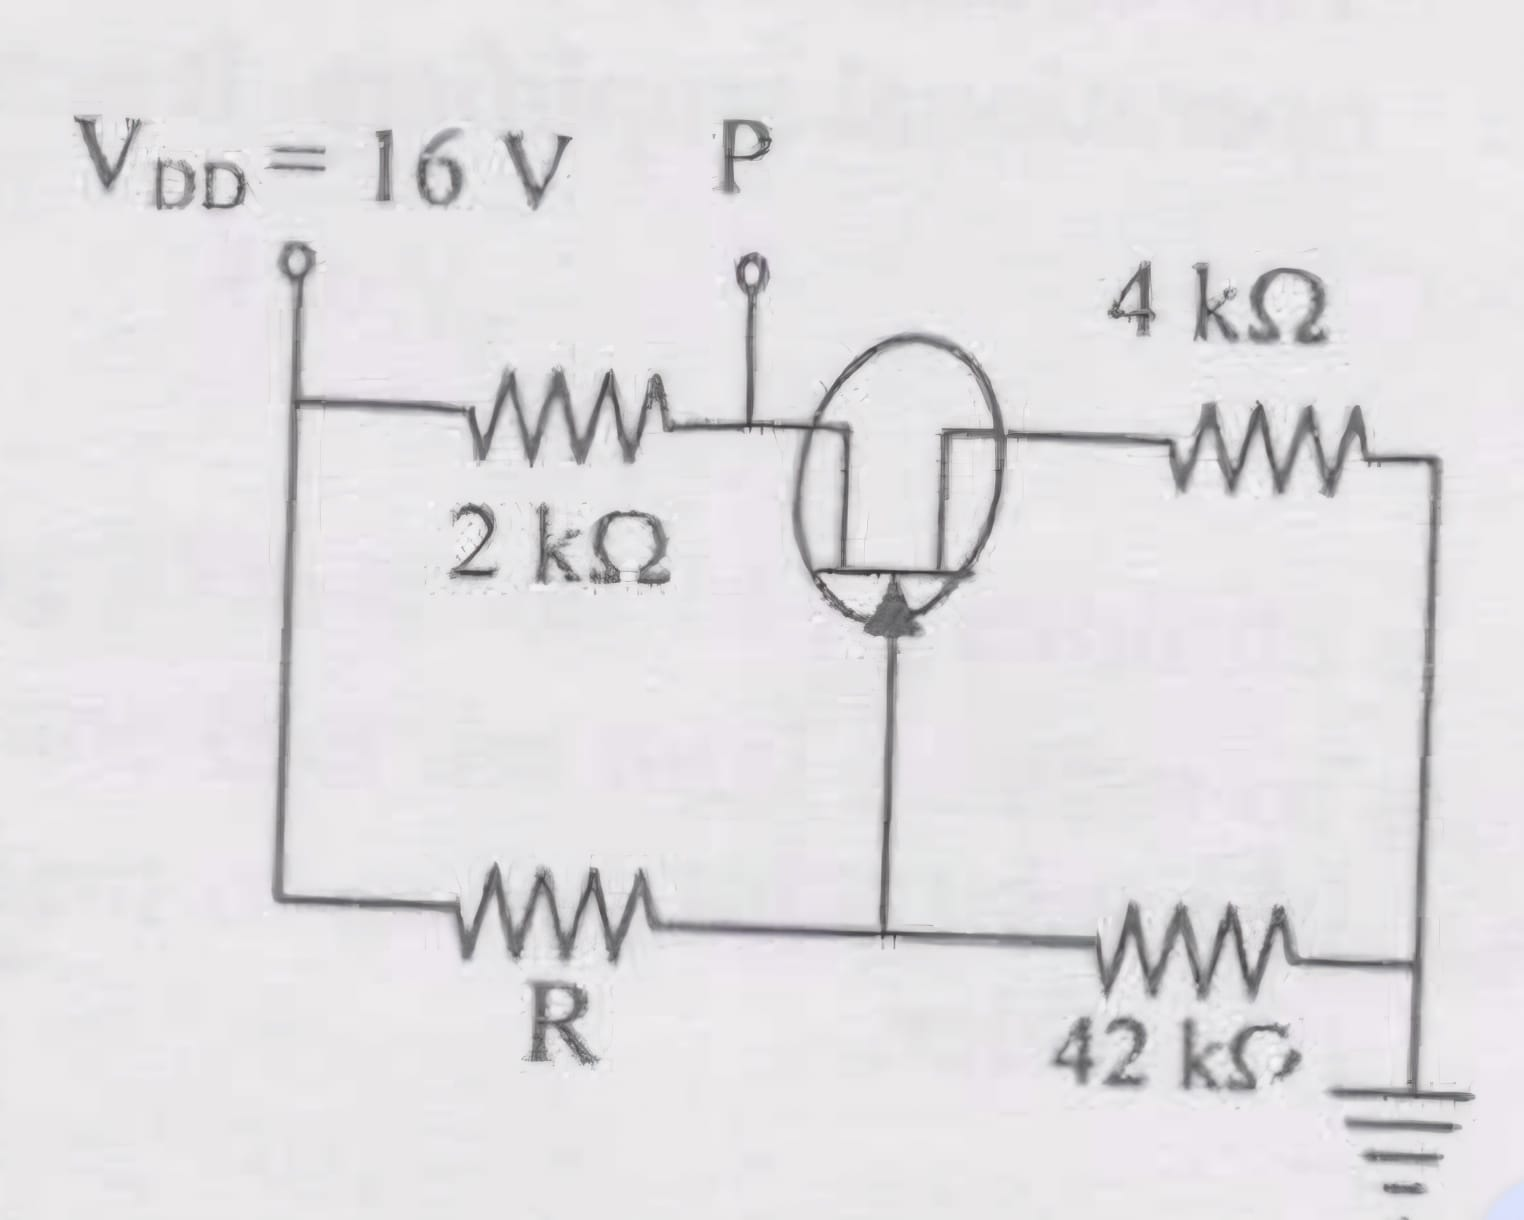
\includegraphics[width=0.25\textwidth]{fig10.jpeg}
    \caption{}
    \label{fig:fig10.jpeg}
\end{figure}

\begin{multicols}{4}
\begin{enumerate}
    \item 42
    \item 48
    \item 56
    \item 70
\end{enumerate} 
\end{multicols}

\item when an input voltage $V_i$, of the form shown, is applied to the circuit given below, the output voltage is of the form

\hfill{\brak{\text{GATE IN 2007}}}

\begin{figure}[ht!]
    \centering
    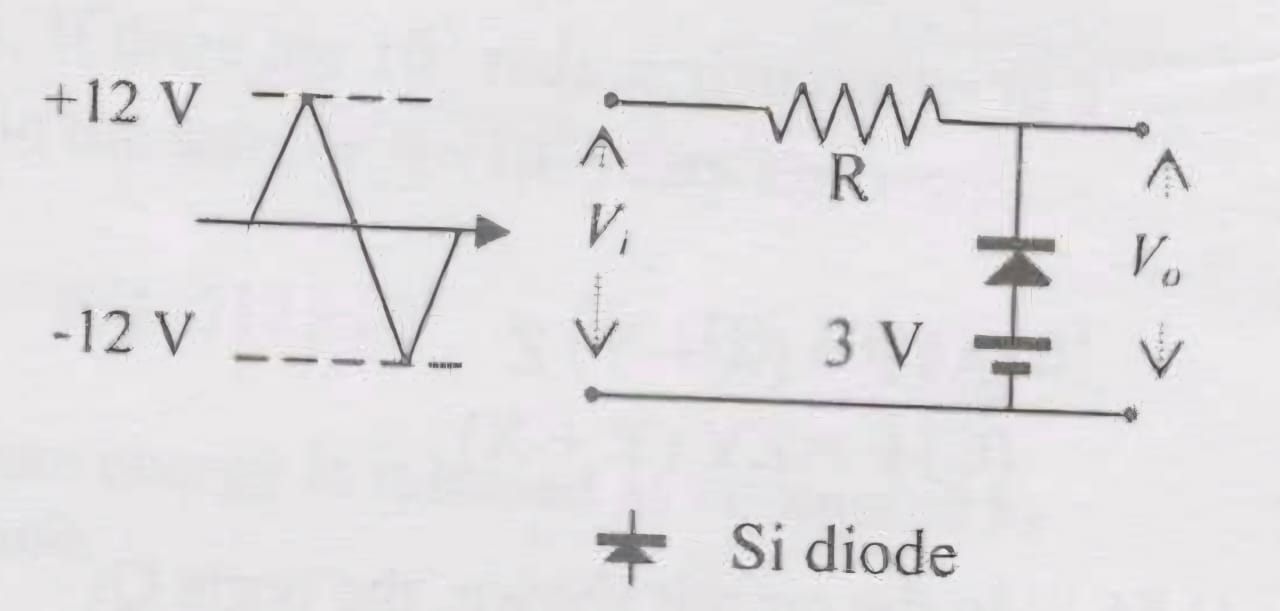
\includegraphics[width=0.5\textwidth]{fig11.jpeg}
    \caption{}
    \label{fig:fig11.jpeg}
\end{figure}
\begin{multicols}{2}
\begin{enumerate}
    \item 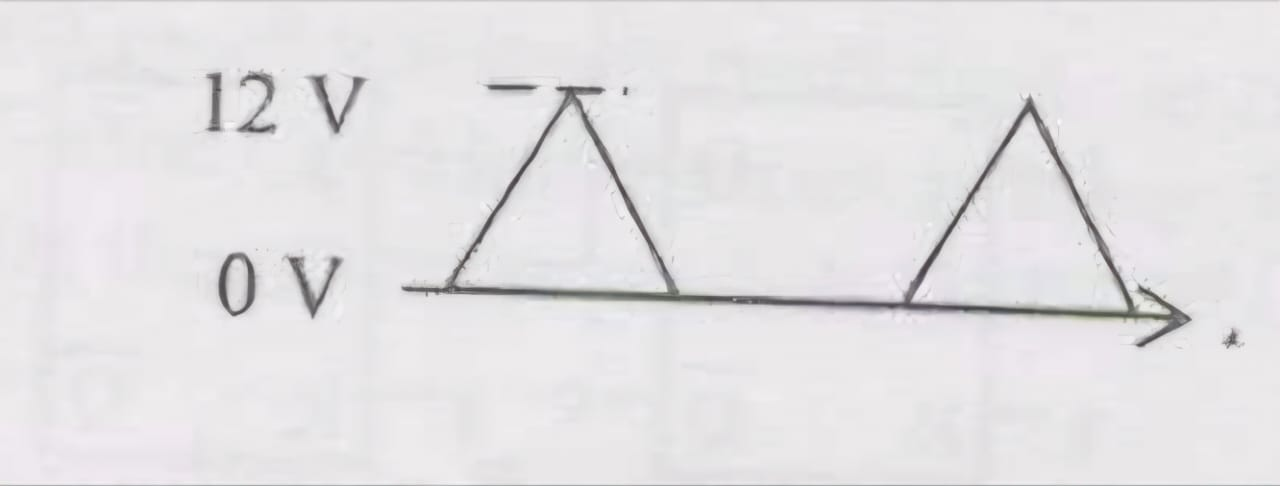
\includegraphics[width=0.25\textwidth]{fig12.jpeg} \hfill
    \item 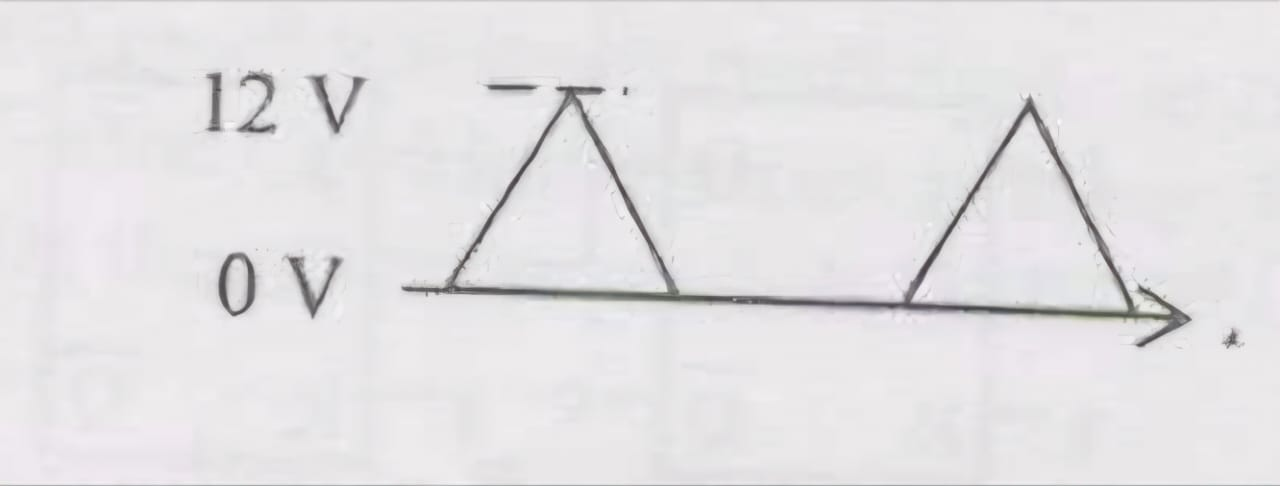
\includegraphics[width=0.25\textwidth]{fig13.jpeg} \hfill
    \item 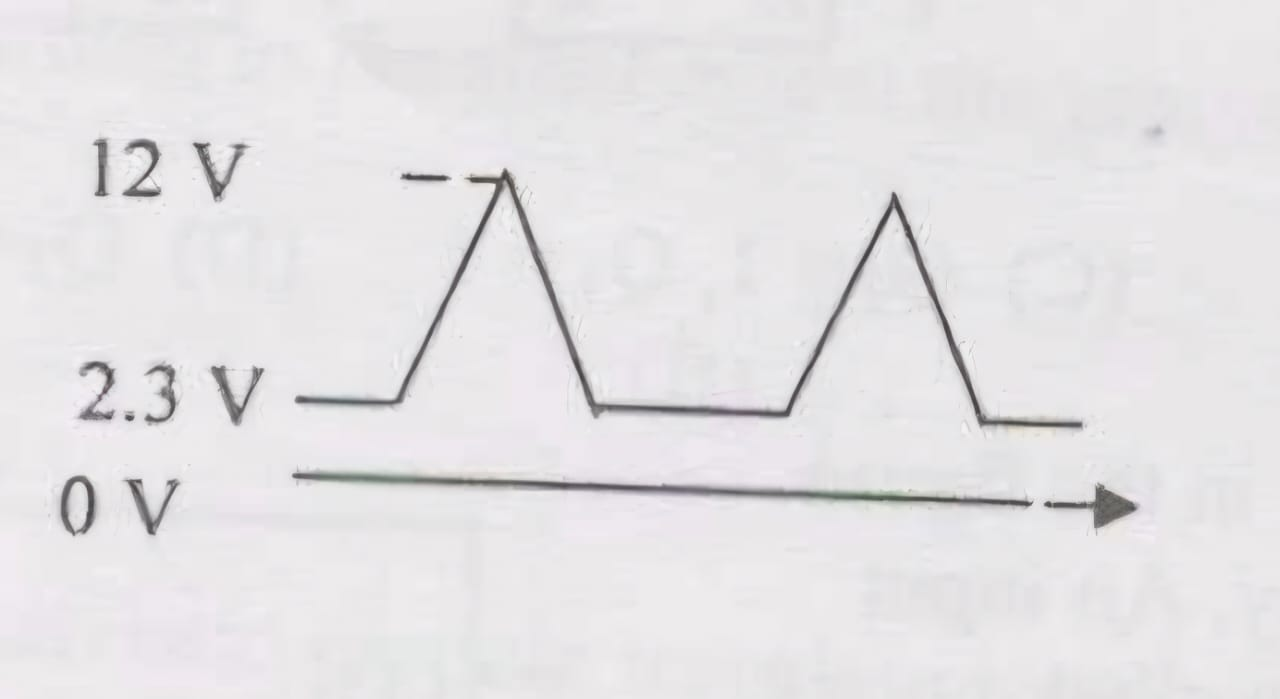
\includegraphics[width=0.25\textwidth]{fig14.jpeg} \hfill
    \item 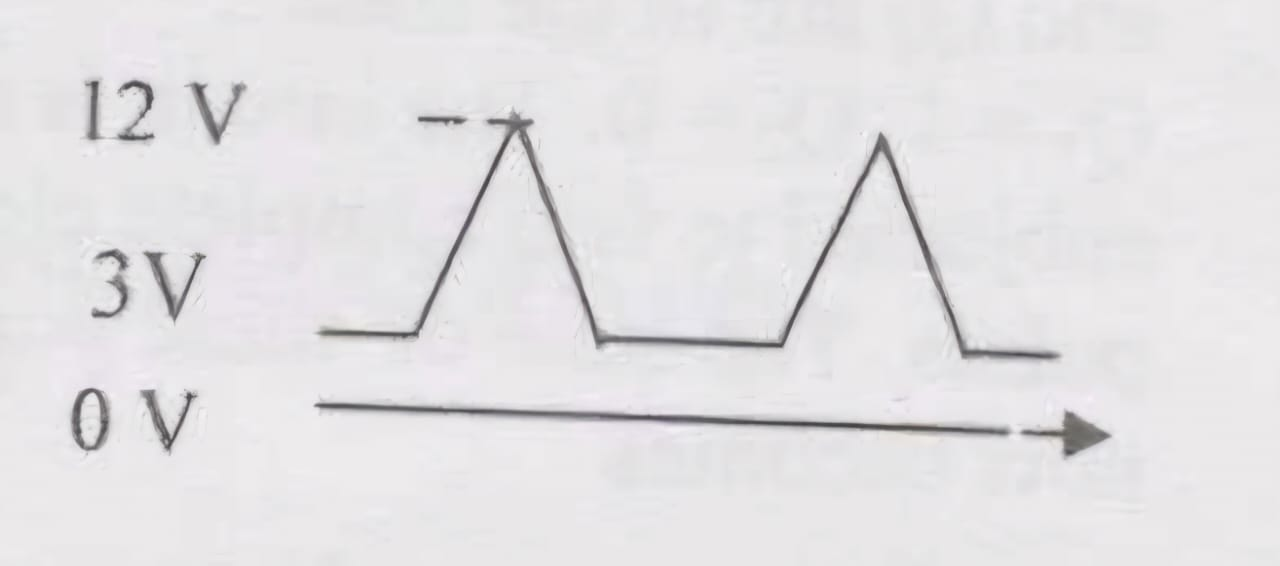
\includegraphics[width=0.25\textwidth]{fig15.jpeg} \hfill
\end{enumerate}
\end{multicols}



\newpage



\begin{center}
\textbf{Common Data Questions}     
\end{center}


\textbf{Common Data for Questions 71,72,73:} \\
A particle of mass $m$ is confined in the ground state of a one-dimensional box, extending from $x=-2L$ to $x=2L$. The wavefunction of the particle in this state is 
$\psi(x) = \psi_A \cos\left(\frac{\pi x}{4L}\right)$, where $\psi_A$ is a constant.


\item The normalization factor of this wavefunction is:

\hfill{\brak{\text{GATE IN 2007}}}

\begin{multicols}{2}
\begin{enumerate}
    \item $\sqrt{2/L}$
    \item $\sqrt{1/(4L)}$
    \item $24$
    \item $\sqrt{1/L}$
\end{enumerate}
\end{multicols}

\item The energy eigenvalue corresponding to this state is:

\hfill{\brak{\text{GATE IN 2007}}}

\begin{multicols}{2}
\begin{enumerate}
    \item $\dfrac{\hbar^2 \pi^2}{2 m L^2}$
    \item $\dfrac{\hbar^2 \pi^2}{4 m L^2}$
    \item $\dfrac{\hbar^2 \pi^2}{16 m L^2}$
    \item $\dfrac{\hbar^2 \pi^3}{32 m L^2}$
\end{enumerate}
\end{multicols}

\item The expectation value of $p^2$ (momentum operator) in this state is:

\hfill{\brak{\text{GATE IN 2007}}}

\begin{multicols}{2}
\begin{enumerate}
    \item $0$
    \item $\dfrac{h^2 \pi^2}{32 L^2}$
    \item $\dfrac{h^2 \pi^3}{16 L^2}$
    \item $\dfrac{h^2 \pi^3}{8 L^2}$
\end{enumerate}
\end{multicols}



\textbf{Common Data for Questions 74,75:} \\
The Fresnel relations between the amplitudes of incident and reflected electromagnetic waves at an interface between air and a dielectric of refractive index $\mu$ are:  
\[
E_\parallel^{\rm ref} / E_\parallel^{\rm inc} = \frac{\cos r - \mu \cos i}{\cos r + \mu \cos i}, \quad
E_\perp^{\rm ref} / E_\perp^{\rm inc} = \frac{\cos i - \mu \cos r}{\cos i + \mu \cos r}
\]  
where $i$ and $r$ are the angles of incidence and refraction respectively.


\item The condition for the reflected ray to be completely polarized is:

\hfill{\brak{\text{GATE IN 2007}}}

\begin{multicols}{2}
\begin{enumerate}
    \item $\mu \cos i = \cos r$
    \item $\cos i = \mu \cos r$
    \item $\mu \cos i = - \cos r$
    \item $\cos i = - \mu \cos r$
\end{enumerate}
\end{multicols}

\item For normal incidence at an air-glass interface with $\mu=1.5$, the fraction of energy reflected is:

\hfill{\brak{\text{GATE IN 2007}}}

\begin{multicols}{2}
\begin{enumerate}
    \item 0.40
    \item 0.20
    \item 0.16
    \item 0.04
\end{enumerate}
\end{multicols}

\newpage
\begin{center}
 \textbf{Linked Answer Questions: Q.76 to Q.81 carry two marks each.}   
\end{center}

\vspace{2em}


\textbf{Statement for Linked Answer Questions 76 \& 77:} \\
In the laboratory frame, a particle $P$ of rest mass $m_0$ is moving in the positive $x$ direction with speed $5c/19$. It approaches an identical particle $Q$, moving in the negative $x$ direction with speed $2c/5$.


\item The speed of the particle $P$ in the rest frame of particle $Q$ is:

\hfill{\brak{\text{GATE IN 2007}}}

\begin{multicols}{4}
\begin{enumerate}
    \item $\dfrac{7c}{95}$
    \item $\dfrac{13c}{85}$
    \item $\dfrac{3c}{5}$
    \item $\dfrac{63c}{95}$
\end{enumerate}
\end{multicols}

\item The energy of the particle $P$ in the rest frame of particle $Q$ is:

\hfill{\brak{\text{GATE IN 2007}}}

\begin{multicols}{4}
\begin{enumerate}
    \item $\dfrac{1}{2} m_0 \omega^2$
    \item $\dfrac{5}{4} m_0 c^2$
    \item $\dfrac{19}{13} m_0 c^2$
    \item $\dfrac{11}{9} m_0 c^2$
\end{enumerate}
\end{multicols}


\vspace{2em}


\textbf{Statement for Linked Answer Questions 78 \& 79:} \\
The atomic density of a solid is $5.85 \times 10^{28} \ \mathrm{m}^{-3}$. Its electrical resistivity is $1.6 \times 10^{-4} \ \Omega\cdot\mathrm{m}$. Assume electrical conduction is described by the Drude model (classical theory), and that each atom contributes one conduction electron.

\item The drift mobility ($\mathrm{m^2 \, V^{-1} s^{-1}}$) of the conduction electrons is:

\hfill{\brak{\text{GATE IN 2007}}}

\begin{multicols}{4}
\begin{enumerate}
    \item $6.67 \times 10^{-3}$
    \item $6.67 \times 10^{-6}$
    \item $7.63 \times 10^{-1}$
    \item $7.63 \times 10^{-4}$
\end{enumerate}
\end{multicols}

\item The relaxation time (mean free time), in seconds, of the conduction electrons is:

\hfill{\brak{\text{GATE IN 2007}}}

\begin{multicols}{4}
\begin{enumerate}
    \item $3.98 \times 10^{-15}$
    \item $3.79 \times 10^{-14}$
    \item $2.84 \times 10^{-12}$
    \item $2.64 \times 10^{-11}$
\end{enumerate}
\end{multicols}

\vspace{2em}

\textbf{Statement for Linked Answer Questions 80 \& 81:} \\
A sphere of radius $R$ carries a polarization $\overline{P} = k \vec{r}$, where $k$ is a constant and $\vec{r}$ is measured from the centre of the sphere.

\item The bound surface and volume charge densities are given, respectively, by:

\hfill{\brak{\text{GATE IN 2007}}}

\begin{multicols}{4}
\begin{enumerate}
    \item $-k |\vec{r}|$ and $3k$
    \item $k |\vec{r}|$ and $-3k$
    \item $k$ and $-4kR$
    \item $-k |\vec{r}|$ and $4kR$
\end{enumerate}
\end{multicols}

\item The electric field $\vec{E}$ at a point outside the sphere is given by:

\hfill{\brak{\text{GATE IN 2007}}}

\begin{multicols}{4}
\begin{enumerate}
    \item $\hat{E} = 0$
    \item $\overline{E} = \dfrac{k R (R^2 - r^2)}{\epsilon_0 r^3} \hat{r}$
    \item $\vec{E} = \dfrac{k R (R^3 - r^2)}{\kappa_a r^3} \hat{r}$
    \item $\vec{E} = \dfrac{3k (r - R)}{4 \pi \epsilon_0 r^4} \hat{r}$
\end{enumerate}
\end{multicols}

\newpage

\textbf{Statement for Linked Answer Questions 82 \& 83:} \\
An ensemble of quantum harmonic oscillators is kept at a finite temperature $T = 1/(k_B \beta)$.

\item The partition function of a single oscillator with energy levels $(m + 1/2)\hbar \omega$ is:

\hfill{\brak{\text{GATE IN 2007}}}

\begin{multicols}{2}
\begin{enumerate}
    \item $Z = e^{-\beta \hbar \omega /2} \frac{1}{1 - e^{-\beta \hbar \omega}}$
    \item $Z = \frac{1}{1 - e^{-\beta \hbar \omega}}$
    \item $Z = e^{-\beta \hbar \omega /2} \frac{1}{1 + e^{-\beta \hbar \omega}}$
    \item $Z = \frac{1}{1 + \mu^{-\beta k_m}}$
\end{enumerate}
\end{multicols}

\item The average number of energy quanta of the oscillators is given by:

\hfill{\brak{\text{GATE IN 2007}}}

\begin{multicols}{2}
\begin{enumerate}
    \item $\langle n \rangle = \frac{1}{e^{2\lambda + \nu} - 1}$
    \item $\langle H \rangle = \frac{e^{-j \lambda x}}{e^{j \lambda x} - 1}$
    \item $\langle n \rangle = \frac{1}{e^{x \lambda x} + 1}$
    \item $\langle n \rangle = \frac{e^{-\beta \beta_w}}{e^{\beta \beta_w \sigma} + 1}$
\end{enumerate}
\end{multicols}


\textbf{Statement for Linked Answer Questions 84 \& 85:} \\
A $16\,\mu\mathrm{A}$ beam of alpha particles, having cross-sectional area $10^{-4}\,\mathrm{m^2}$, is incident on a rhodium target of thickness $1\,\mu\mathrm{m}$. This produces neutrons through the reaction:  
\[
\alpha + {}^{100}\mathrm{Rh} \rightarrow {}^{100}\mathrm{Pd} + 3n
\]

\item The number of alpha particles hitting the target per second is:

\hfill{\brak{\text{GATE IN 2007}}}

\begin{multicols}{2}
\begin{enumerate}
    \item $0.5 \times 10^{14}$
    \item $1 \times 10^{14}$
    \item $2 \times 10^{10}$
    \item $4 \times 10^{11}$
\end{enumerate}
\end{multicols}

\item The neutrons are observed at the rate of $1.306 \times 10^4 \ \mathrm{s^{-1}}$. If the density of rhodium is approximated as $10\,\mathrm{kg/m^3}$, the cross-section (in barns) is:

\hfill{\brak{\text{GATE IN 2007}}}

\begin{multicols}{2}
\begin{enumerate}
    \item $0.1$
    \item $0.2$
    \item $0.4$
    \item $0.8$
\end{enumerate}
\end{multicols}

\end{enumerate}


\begin{center}
 \textbf{END OF THE QUESTION PAPER}   
\end{center}


\vspace{2cm}
\textbf{Space for Rough Work:} \\


\end{document}
